\documentclass[tikz,border=10pt]{standalone}

\usetikzlibrary{arrows}
\usepackage{upquote}

\definecolor{apricot}{rgb}{0.98, 0.81, 0.69}
\definecolor{persimmon}{rgb}{0.93, 0.35, 0.0}
\definecolor{orange-red}{rgb}{1.0, 0.27, 0.0}

\begin{document}
\nopagecolor

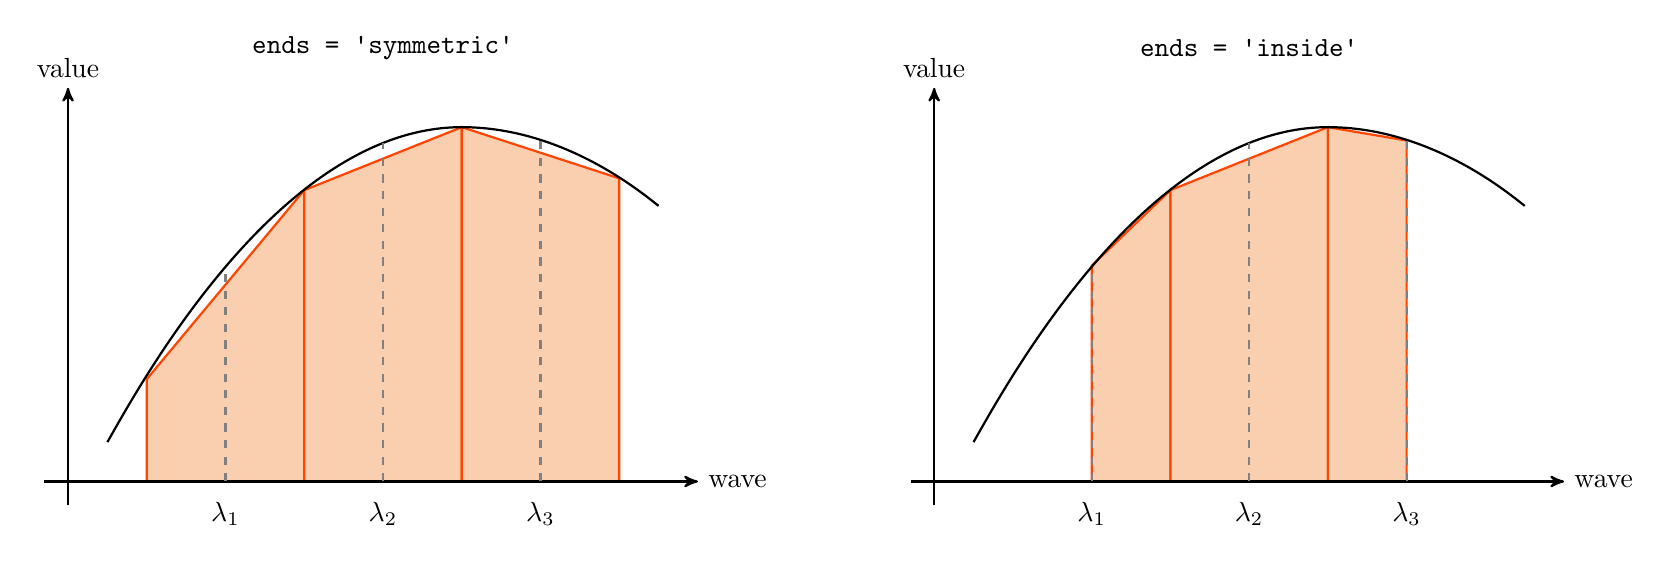
\begin{tikzpicture}[
    scale=1,
    thick,
    >=stealth']
   
    \node at (4,5.5) {\verb|ends = 'symmetric'|};

    \draw [draw=orange-red, fill=apricot] (1,0) -- (1,1.3) -- (3,3.7) -- (3,0) -- cycle;
    \draw [draw=orange-red, fill=apricot] (3,0) -- (3,3.7) -- (5,4.5) -- (5,0) -- cycle;
    \draw [draw=orange-red, fill=apricot] (5,0) -- (5,4.5) -- (7,3.85) -- (7,0) -- cycle;
    
    \draw[->] (-0.3,0) -- (8,0) coordinate[label = {right:wave}];
    \draw[->] (0,-0.3) -- (0,5) coordinate[label = {above:value}];
    \draw (0.5,0.5) parabola bend (5,4.5) (7.5,3.5);

    \draw [gray, dashed] (2,0) node[label=below:{\color{black}$\lambda_1$}]{} -- (2,2.74);
    \draw [gray, dashed] (4,0) node[label=below:{\color{black}$\lambda_2$}]{} -- (4,4.3);
    \draw [gray, dashed] (6,0) node[label=below:{\color{black}$\lambda_3$}]{} -- (6,4.33);


    % ends

    \node at (15,5.5) {\verb|ends = 'inside'|};

    \draw [draw=orange-red, fill=apricot] (13,0) -- (13,2.74) -- (14,3.7) -- (14,0) -- cycle;
    \draw [draw=orange-red, fill=apricot] (14,0) -- (14,3.7) -- (16,4.5) -- (16,0) -- cycle;
    \draw [draw=orange-red, fill=apricot] (16,0) -- (16,4.5) -- (17,4.33) -- (17,0) -- cycle;
    
    \draw[->] (10.7,0) -- (19,0) coordinate[label = {right:wave}];
    \draw[->] (11,-0.3) -- (11,5) coordinate[label = {above:value}];
    \draw (11.5,0.5) parabola bend (16,4.5) (18.5,3.5);

    \draw [gray, dashed] (13,0) node[label=below:{\color{black}$\lambda_1$}]{} -- (13,2.74);
    \draw [gray, dashed] (15,0) node[label=below:{\color{black}$\lambda_2$}]{} -- (15,4.3);
    \draw [gray, dashed] (17,0) node[label=below:{\color{black}$\lambda_3$}]{} -- (17,4.33);


\end{tikzpicture}

\end{document}
